\documentclass[a4paper, 12pt, italian]{report}
\usepackage{ctable}
\usepackage{url}
\usepackage[utf8]{inputenc}
\usepackage{enumitem}
\usepackage{graphicx}
\usepackage{longtable}
\usepackage{amsmath}
\usepackage[italian]{babel}

\usepackage[raggedright]{titlesec}
\usepackage{blindtext}

\titleformat{\chapter}[hang]{\bfseries\huge}{\thechapter.}{2pc}{}
\titlelabel{\thetitle.\quad}   % For consistency in all headings

\begin{document}
\begin{titlepage}
\newcommand{\HRule}{\rule{\linewidth}{0.5mm}} 
\center 
\textsc{\LARGE Università degli studi di Salerno}\\[1cm] 

\includegraphics[width=3.5cm]{img/logo.jpg} \\[1cm]
\textsc{\large Progetto di Ingegneria del Software II}\\[0.5cm]
\textsc{\Large Repominer Evolution}\\[0.5cm] 
 \HRule \\[0.4cm]
{ \large \bfseries Software Project Management Plan}\\[0.4cm] 
\HRule \\[1.5cm]

\begin{minipage}{0.4\textwidth}
\begin{flushleft} \large
\emph{Autori:}\\
Matteo \textsc{Merola}\\
Carlo \textsc{Branca}\\
Simone \textsc{Scalabrino}\\
Giovanni \textsc{Grano}\\
\end{flushleft}
\end{minipage}
~
\begin{minipage}{0.4\textwidth}
\begin{flushright} \large
\emph{Supervisore:} \\
Prof. Andrea \textsc{De Lucia}
\end{flushright}
\end{minipage}\\[2.5cm]

{\Large SPMP}\\
Versione 1.0\\[1cm]

{\large 15 maggio 2014} % Date, change the \today to a set date if you want to be precise

\vfill

\end{titlepage}		
       \chapter*{Revision History}

\ctable[
    caption = Tabella delle revisioni del documento,
    label   = width,
    width   = 145mm,
    pos     = ht
 ]{ccc>{\raggedright}X}{}
 { 
\FL
\multicolumn{1}{c}{Data} &\multicolumn{1}{c}{Versione}&\multicolumn{1}{c}{Descrizione}&\multicolumn{1}{c}{Autori}\ML
 14/07/2014 &
 1.0 &
 Versione iniziale&
 Simone Scalabrino, Giovanni Grano, Carlo Branca, Matteo Merola 
 \LL
}
	\setcounter{tocdepth}{1}	
	\tableofcontents
	\listoffigures
	\listoftables
	
	\chapter{Introduzione}

\section{Scopo del documento}
		
Il presente documento, oltre a fornire una panoramica del progetto, descrive il processo di management che sarà portato avanti durante le fasi progettazione e sviluppo. Il documento sarà aggiornato in maniera iterativa per offrire informazioni più precise riguardo le diverse fasi del progetto. 


\section{Evoluzione del presente documento}

Allo stato attuale del progetto, molte informazioni nel SPMP risultano incomplete o poco precise. Il documento sarà aggiornato e rivisto con l'avanzare dei lavori in modo da garantire una completa descrizione del processo manageriale condotto.


\section{Definizioni ed acronimi}

Definizioni:			
\begin{itemize}
\item \emph{Deliverables}: con il termine deliverables si ci riferisce generalmente alla documentazione tecnico/commerciale da consegnare al cliente quale risultato dell'esecuzione di una o più fasi di un progetto.
\item \emph{Scheduling}: pianificazione dei tempi e delle precedenze nell'impiego di risorse materiali ed umane per un buon svolgimento del processo di progettazione e sviluppo di un sistema software.
\item \emph{Work breakdown structure (WBS)}: rappresentazione di un progetto che consiste in una strutturazione tipicamente gerarchica delle attività che lo compongono in sotto-attività fino ad un opportuno livello di approfondimento.
\item \emph{Diagramma di Gantt}: strumento di supporto alla gestione dei progetti utilizzato principalmente nell'attività di project management quale rappresentazione dello scheduling delle attività o mansioni che costituiscono un progetto.
\end{itemize}	

Acronimi:
\begin{itemize}
\item \emph{ODD}: Object Design Document
\item \emph{WBS}: Work Breakdown Structure
\end{itemize}
	\chapter{Panoramica}

In riferimento al ciclo di vita del software, è chiaro osservare come, una volta che il prodotto viene rilasciato, andrà incontro per forza di cose a diverse modifiche per i più svariati motivi, dalla correzione di errori all'estensione di funzionalità. Tale concetto viene espresso dalla prima legge di Lehman dulla manutenzione del software:
\begin{center}
\textit{un sistema deve necessariamente cambiare ed evolvere con continuità per mantenere intatto il suo livello di utilità, stante i continui cambiamenti che avvengono nell'ambiente in cui il sistema opera}.
\end{center}
Quando un sistema cambia, per qualsivoglia motivo, la tua struttura tende a diventare più complessa. Diventa necessario utilizzare risorse supplementari per preservarne la qualità della struttura. Assume importanza estrema quindi il monitorare la qualità del codice attraverso l'utilizzo di metriche.\\

Nell'Ingegneria del software, la predizione dei faults è stata sempre comunemente associata a misurazioni di complessità. Il concetto di entropia più essere applicato con successo in diversi contesti, a partire dal concetto di defect prediction. L'idea di base è quella di proporre metriche complesse che sono basate sul processo di cambiamento del codice invece che sul codice stesso. Si può ragionevolemente congetturare come, un processo di cambiamento complesso e disomogeneo, possa affliggere negativamente un sistema software. 

Proprio come strumento per quantificare la complessità ritorna utile il concetto di entropia di Shannon. A partire da queste informazioni è possibile andare ad implementare due modelli per la complessità dei cambiamenti sul codice; il \textit{Basic Code Change Model} e un modello più elaborato e complesso, il \textit{Extended Code Change Model}. Entrambi questi modelli vanno a calcolare un singolo valore che misura la complessità complessiva dei cambiamenti di un progetto durante un periodo di tempo stabilito. 

Come mostrato nel caso di studio svolto nel lavoro di Hassan, tali metriche basate sulla complessità dei cambiamenti si rivelavano estremamente valide nella defeat prediction.\\

Occore specificare come, in questi modelli, si andranno ad analizzare solamente le cosiddette FI, ossia \textit{Features Introduction Modifications}; per FI intendiamo modifiche al codice che vanno ad implementare nuove features nel sistema. In questa categoria andrà a confluire tutto ciò che non può essere catalogato come FR (\textit{Fault Repairing Modifications}) e come GM (\textit{General Maintenance Modifications}). Come unità da misurare si è scelto il singolo file, in quanto si può ragionevolmente credere che è nel file che i developers concentrano e raggruppano le singole entità.\\

Come già detto, il modello BCC utilizza un arco temporale ben specificato, e definisce, file per file, la probabilità che lo stesso subisca un cambiamento. Più le probabilità sono equamente distribuite, più alta è l'entropia del sistema software, e dunque maggiore è la probabilità di svilupare difetti. Come caso limite invece, qualora un singolo file raggiunga probabilità 1, abbiamo che l'entropia del sistema diviene minima. L'idea chiave dunque risiede nel focalizzare l'analisi sulle modifiche alla singole linee di codice lungo un intervallo di tempo, allo scopo di costruire un modello di probabilità dei cambiamenti.

Quest'analisi fornisce ovviamente anche un andamento evolutivo di quella che è l'entropia del sistema lungo tutto il suo ciclo di vita. Partizionando lo stesso in periodi successivi di tempo, è interessante notare come il processo di cambiamento del codice si sia evoluto e protratto nel tempo di pari passo all'entropia dello stesso. Ciò costituisce anche un'importante parametro di monitoraggio per un manager. Si è osservato come, individuando le ragioni di picchi inaspettati nell'entropia, sia possibile pianificare ed essere pronti per problemi futuri.\\

Nel BCC sin qui descritto a grandi linee si assume un intervallo di tempo fissato per il calcolo dell'entropia, e si assume che il numero di file in un sistema rimanga inalterato. Ovviamente queste limitazioni restringono in campo di utilizzo di questo modello. L'\textit{Extended Code Change} va a colmare tali lacune. In particolare, per quanto riguarda l'arco di tempo da analizzare nell'evoluzione software, è possibile prendere in considerazione diverse opzioni differenti. Abbiamo già visto il criterio del \textit{time based periods}, ossia la suddivisione in parti eque dei periodi di tempo, a partire dall'inizio del progetto fino alla sua conclusione. Si crede che un periodo di periodo di un quarto di anno sia un limite di tempo ragionevole per raccogliere una frazione significativa nella crescita di un sistema. Un'altra possibilità riguarda i \textit{modification limit base periods}, ossia il suddividere il tempo in periodi basandosi sul numero di modifiche che sono memorizzare nella repository in oggetto. Per prevenire i casi in cui si verificano lunghi periodi di scarse modifiche implementative, è ragionevole imporre un limite temporale di 3 mesi qualora un periodo non raggiunga un limite fissato a 600 modifications. In conclusione, si è osservato come il processo di modifica segua delle fasi di picco, seguire da fasi di rilassamento. È sulla base di questa osservazione che è possibile la suddivisione temporale in \textit{burst based periods}.\\

Nel modello ECC è necessario definire un'entropia normalizzata, con lo scopo di comparare l'entropia di sistemi di differente dimensione, con aggiunta o rimozione di files durante i vari periodi di tempo. La \textit{normalized static entropy} \textit{H} dipende dal numero di files in un sistema. È interessante notare alcuni sistemi software annoverino alcuni files con una probabilità di cambiamento davvero bassa. Per fare in modo che questi files non riducano in maniera artificiosa l'entropia del sistema, si è definita l'\textit{adaptive sizing entropy}. L'idea di fondo è quella di dividere per il numero di linee recentemente modificate, invece per il numero attuale di linee del sistema. Vi sono due criteri di scelta per calcolare tale valore, ossia un primo criterio che prende in esame i files modificati nei precedenti \textit{x} mesi,incluso il mese corrente, mentre un secondo prevede che il set di files da analizzare includa tutti i files modificati nei precedenti \textit{x} periodi, incluso quello corrente. 
	\chapter{Organizzazione del progetto}	
		
		\section{Organizzazione strutturale}
		\label{sec:struc}
		
		La struttura organizzativa del progetto risulta difficile da stabilire in questa fase preliminare. In fasi più avanzate, i team member potranno essere suddivisi in team dedicati ad attività specifiche (Es. team di implementazione, team di testing).
		
		\begin{figure}[ht]
		\centering
		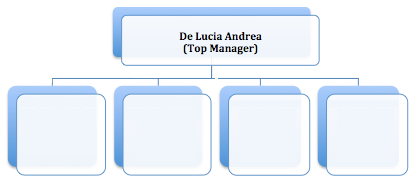
\includegraphics[width=\textwidth]{img/organizzazione.png}
		\caption{Struttura organizzativa}\label{fig:1}
		\end{figure}
		
		\begin{table}[ht]
		\centering
			\begin{tabular}{|c|c|c|}
				\hline
				\textbf{Nome componente} & \textbf{Ruolo} & \textbf{Responsabilità}\\
				\hline
				Matteo Merola & Team member & \shortstack{Sviluppo deliverables:\\DL1, DL2, DL3}\\
				\hline
				Simone Scalabrino & Team member &  \shortstack{Sviluppo deliverables:\\DL1, DL2, DL3}\\
				\hline
				Giovanni Grano & Team member & \shortstack{Sviluppo deliverables:\\DL1, DL2, DL3}\\
				\hline
				Carlo Branca & Team member & \shortstack{Sviluppo deliverables:\\DL1, DL2, DL3}\\
				\hline
			\end{tabular}
		\caption{Ruoli e responsabilità}
		\label{proj_org:ruoli}
		\end {table}
		
	\chapter{Scheduling delle attività}
\section{Tabella di scheduling}
La tabella \ref{activity:scheduling} mostra lo scheduling delle macro-attività previsto.

\newcolumntype{C}[1]{>{\centering}p{#1}}
\begin{table}[ht]
	\centering
	\begin{tabular}{|C{2cm}|C{3cm}|C{2cm}|C{2cm}|C{2.5cm}|}
	\hline
	\textbf{Codice attività}	& \textbf{Nome attività}	& \textbf{Data inizio}	& \textbf{Data fine}		& \textbf{Codici deliverable}\tabularnewline
	\hline
	
	AC0		&	Analisi					&	15/05/2014	&	19/05/2014	& DL2\tabularnewline
	
	\hline
	
	AC1		&	Pianificazione testing	&	20/05/2014	&	1/06/2014	& DL4, DL5\tabularnewline
	
	\hline
	
	AC3		&	ODD						&	20/05/2014	&	9/07/2014	& DL3\tabularnewline
	
	\hline
	
	AC4		&	Primo incremento		&	20/05/2014	&	5/06/2014	& DL6, DL7\tabularnewline
	
	\hline
	
	AC5		&	Secondo incremento		&	 1/06/2014	&	28/06/2014	& DL8, DL9\tabularnewline
	
	\hline
	
	AC6		&	Terzo incremento		&	23/06/2014	&	7/07/2014	& DL10, DL11\tabularnewline
	
	\hline
	
	AC7		&	Management				&	28/04/2014	&	13/07/2014	& DL1, DL12\tabularnewline
	
	\hline
	\end{tabular}
	
	\caption{Scheduling delle attività}
	\label{activity:scheduling}
\end{table}

\clearpage
\section{Work Breakdown Structure (WBS)}
In questa sezione è presentata la WBS del progetto e le WBS dettagliate per documento di analisi, ODD e documentazione di testing; in particolare, per le WBS della documentazione vengono presentati due formati: l'org-chart format e l'outline format.

Nell'org-chart format vengono rappresentate le componenti principali che sono dettagliate nell'outline format per questione di spazio.
\subsection{WBS progetto}
\begin{figure}[ht]
\centering
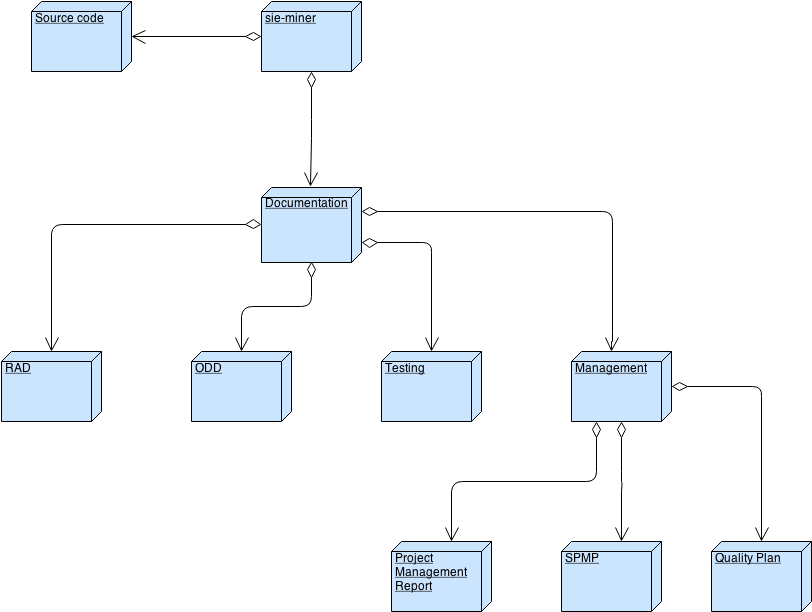
\includegraphics[width=\textwidth]{img/WBS_master.png}
\caption{WBS RepoMinerEvo} 
\end{figure}
\clearpage

% WBS Analisi ---------------------

\subsection{WBS Documento di analisi}
\begin{figure}[ht]
\centering
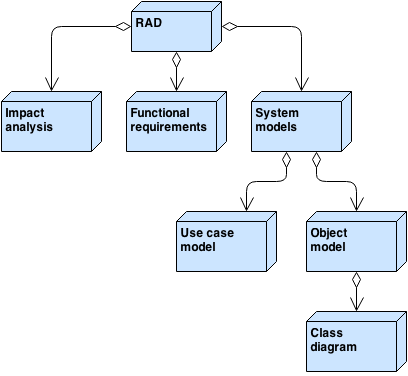
\includegraphics[width=.5\textwidth]{img/wbs_rad.png}
\caption{WBS Documento di analisi} 
\end{figure}
\textbf{WBS Documento di analisi - Outline format:}
\begin{enumerate}
\item Introduzione
\begin{enumerate}[label*=\arabic*.]
\item Scopo del sistema
\item Definizioni, acronimi, abbreviazioni
\item Panoramica
\item Sistema corrente
\end{enumerate}
\item Sistema proposto
\begin{enumerate}[label*=\arabic*.]
\item Requisiti funzionali
\end{enumerate}
\item System Model
\begin{enumerate}[label*=\arabic*.]
\item Use case models
\item Object models
\end{enumerate}
\item Impact analysis
\item Glossario
\end{enumerate}
\clearpage

% WBS ODD ---------------------
\subsection{WBS ODD}
\begin{figure}[ht]
\centering
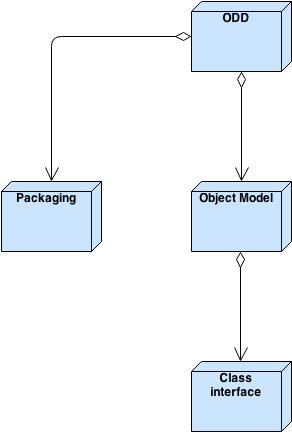
\includegraphics[width=.5\textwidth]{img/ODD.png}
\caption{WBS ODD} 
\end{figure}
\textbf{WBS ODD - Outline format:}
\begin{enumerate}
\item Introduzione
\begin{enumerate}[label*=\arabic*.]
\item Trade off dell'object design
\item Linee guida per la documentazione delle interfacce
\item Definizioni, acronimi e abbreviazioni
\item References
\end{enumerate}
\item Package
\begin{enumerate}[label*=\arabic*.]
\item Package
\item Comunicazione tra i package
\item Classi e interfacce nei package
\end{enumerate}
\item Object Model
\begin{enumerate}[label*=\arabic*.]
\item Interfaccia delle classi
\end{enumerate}
\item Glossario
\end{enumerate}
\clearpage

% WBS testing ---------------------
\subsection{WBS testing}
\begin{figure}[ht]
\centering
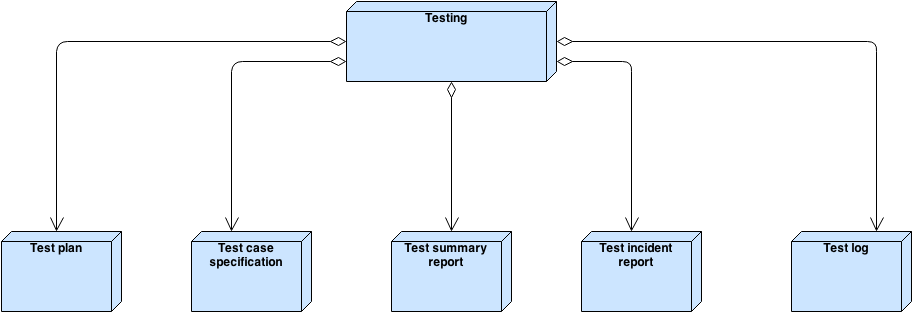
\includegraphics[width=\textwidth]{img/WBS_testing.png}
\caption{WBS Testing} 
\end{figure}
\textbf{WBS ODD - Outline format:}\\ \\
\textbf{Test Plan}:
\begin{enumerate}
\item Introduzione
\item Relazioni con altri documenti
\item Panoramica del sistema
\item Funzionalità da testare/non testare
\item Pass/Fail criteria
\item Approccio
\item Sospensione e ripristino
\item Strumenti per il testing (hardware e software)
\item Test case
\item Pianificazione del test
\end{enumerate}
\clearpage

\section{Diagramma di Gantt}
Il diagramma di Gantt riportato in figura \ref{gantMain} rappreenta lo scheduling delle attività elencate nella sezione 4.1 del presente documento
\begin{figure}[ht]
\centering
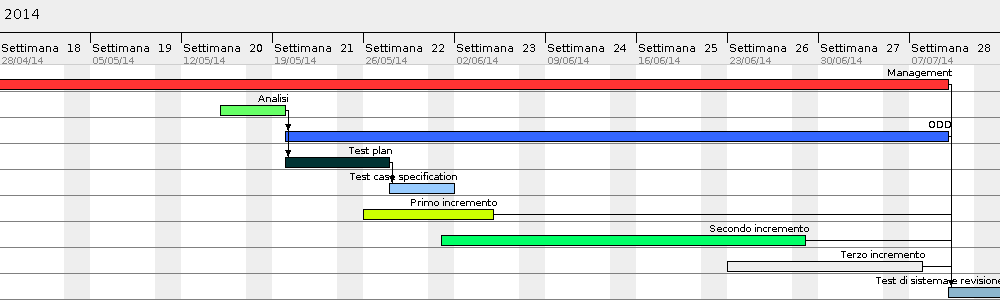
\includegraphics[width=\textwidth]{Gantt/Generic.png} 
\caption{Diagramma di Gantt scheduling delle attività}
\label{gantMain}
\end{figure}

Di seguito le principali scandenze:
\begin{itemize}
\item 19/05/14: Consegna Documento di analisi
\item 27/05/14: Consegna Test Plan
\item 01/06/14: Consegna Test case specification
\item 04/06/14: Termine primo incremento d'implementazione
\item 28/06/14: Termine secondo incremento d'implementazione
\item 07/07/14: Termine terzo incremento d'implementazione
\item 13/07/14: Termine fase di test di sistema e revisione
\end{itemize}

	\chapter{Analisi dei rischi}
\section{Identificazione dei rischi}
In questa sezione sono identificati i possibili problemi cui il progetto potrebbe andare incontro. Per ogni rischio è indicata la probabilità attesa che si verifichi e l'impatto sulla riuscita del progetto. A seguire, nella sezione 5.2, le strategie adottate per ridurre l'impatto dei rischi sul progetto e le azioni da intraprendere nell'eventualità che un rischio si verifichi.
\\ \\
\textbf{Legenda} \\ \\
\textit{Probabilità}:
\begin{itemize}
\item \textit{Bassa}:la probabilità che il rischio si verifichi è compresa nell'intervallo 0\%-30\%.
\item \textit{Media}:la probabilità che il rischio si verifichi è compresa nell'intervallo 30\%-60\%.
\item \textit{Alta}:la probabilità che il rischio si verifichi è compresa nell'intervallo 60\%-100\%.
\end{itemize}
\textit{Impatto}:
\begin{itemize}
\item \textit{Insignificante}: il verificarsi del rischio non compromette la buona riuscita del progetto.
\item \textit{Tollerabile}: classifica rischi di semplice gestione in quanto, le problematiche ad essi collegate, sono facilmente risolvibili.
\item \textit{Serio}: rischi di questo tipo possono rallentare notevolmente il progetto mettendone a rischio la buona riuscita; è necessario risolverli nel più breve tempo possibile.
\item \textit{Catastrofico}: rischi di difficile soluzione; se non affrontati per tempo portano di sicuro al fallimento.
\end{itemize}

\newcolumntype{C}[1]{>{\centering}p{#1}}
\begin{table}[ht]
\centering
\begin{tabular}{|C{3cm}|C{3cm}|C{3cm}|}
\hline 
\textbf{Rischio} & \textbf{Probabilità} & \textbf{Impatto} \tabularnewline
\hline 
Skill del team insufficienti & Bassi & Tollerabile \tabularnewline
\hline
Poca conoscenza del dominio applicativo & Media & Serio \tabularnewline
\hline
Perdita di un elemento del team & Bassa & Tollerabile \tabularnewline
\hline
Ritardo consegna task & Media & Tollerabile \tabularnewline
\hline
Implementazione non completa & Bassa & Serio \tabularnewline
\hline
Attività prolungata oltre la scadenza prevista in fase di schedule & Media & Serio \tabularnewline
\hline
Incontro settimanale annullato & Bassa & Tollerabile \tabularnewline
\hline
\end{tabular}
\caption{Identificazione dei rischi}
\end{table}

\section{Strategie adottate nel risk management}
\textsc{Skill del team insufficienti}
\begin{itemize}
\item \textit{Prevenzione}: assegnare un task con maggior coefficiente di difficoltà ai membri più preparati. Assegnare task particolari a membri del team che hanno acquisito già in precedenza una particolare skill. Durante lo svolgimento dei meeting, cercare di fornire informazioni dettagliate sullo svolgimento dei task assegnati: definire input, lavoro da svolgere e output desiderato, fornendo eventualmente riferimenti su materiale utile per lo svolgimento del task.
\item \textit{Piano di contingenza}: privilegiare task di gruppo affiancando membri del team più preparati a coloro che mostrano maggiori lacune.
\end{itemize}
\textsc{Poca conoscenza del dominio applicativo}
\begin{itemize}
\item \textit{Prevenzione}: prestare particolare attenzione nei meeting iniziali a discutere con il gruppo ogni aspetto del progetto, chiarendo eventuali dubbi, sottolineandone l'utilità e il dominio applicativo in cui va a posizionarsi. 
\item \textit{Piano di contingenza}: dedicare incontri straodinari alle discussioni inerenti il dominio applicativo. Domandare chiarimenti agli sviluppatori del progetto originale.
\end{itemize}
\textsc{Perdita di un elemento del team}
\begin{itemize}
\item \textit{Prevenzione}: assegnare task complicati, quali l'implementazione, a coppie di membri del team, riducendo così il danno nel caso di verificarsi del rischio. Formare un gruppo omogeneo per quanto riguarda obbiettivi e aspettative sul lavoro da svolgere.
\item \textit{Piano di contingenza}: ridistribuire i task lasciati in sospeso dal membro uscente del team tra le risorse ancora a disposizione. Considerare eventuali modifiche allo scheduling.  
\end{itemize}
\textsc{Ritardo nella consegna del task}
\begin{itemize}
\item \textit{Prevenzione}: fornire incentivi alle risorse nel caso di consegna puntuale del task, penalizzazioni altrimenti. In sede di meeting iniziali far notare che un ritardo su un task potrebbe causare un ritardo nella consegna del progetto collettivo, e quindi un danno per tutti i singoli elementi del team.
\item \textit{Piano di contingenza}: assegnare task più impegnativi a membri del team che dimostrano puntualità nella consegna; considerare eventuali modifiche allo scheduling.
\end{itemize}
\textsc{Implementazione non completa}
\begin{itemize}
\item \textit{Prevenzione}: valutare attentamente il monte ore a disposizione nello stabilire i moduli del sistema da implementare, tenendo conto anche delle esigenze dei membri del team.
\item \textit{Piano di contingenza}: documentare le difficoltà incontrare e motivare il verificarsi del rischio.
\end{itemize}
\textsc{Attività prolungata oltre la scadenza prevista in fase di schedule}
\begin{itemize}
\item \textit{Prevenzione}: monitorare attentamente i progressi del progetto lungo la sua durata.
\item \textit{Piano di contingenza}: riformulare lo schedule ed inviduare possibili attività sulle quali recuperare il ritardo accumulato. Se il ritardo è così grave da pregiudicare la consegna finale del progetto, valutare la possibilità di procrastinarne la stessa.
\end{itemize}
\textsc{Incontro settimanale annullato}
\begin{itemize}
\item \textit{Prevenzione}: stabilire gli incontri settimanalmente in accordo alle necessità e alla disponibilità di tutti i membri del team.
\item \textit{Piano di contingenza}: recuperare l'incontro o affidarsi a mezzi di comunicazione sincrona disponibili sul web.
\end{itemize}


\end{document}
